% Slides for 2025-02-10
% To create a slide, use the following:
% \begin{frame}{TITLE}
%     BODY
% \end{frame}

% To create a slide with a bullet list, use the following:
% \begin{frame}{TITLE}
%     \begin{itemize}
%         \item ITEM 1
%         \item ITEM 2
%     \end{itemize}    
% \end{frame}

% To create a slide with numbered list, use the following:
% \begin{frame}{TITLE}
%     \begin{enumerate}
%         \item ITEM 1
%         \item ITEM 2
%     \end{enumerate}
% \end{frame}

% To create a slide with a graphic:
% 1. Add the graphic to this folder (named picture.png)
% 2. Use the following:
% \begin{frame}{TITLE}
%     \centering
%     \includegraphics[height=0.7\textheight,width=0.7\textwidth,keepaspectratio]{picture.png}
% \end{frame}

% To create a slide with two columns, use the following:
% \begin{frame}{TITLE}
%     \begin{columns}
%         \begin{column}{0.5\textwidth}
%             COLUMN 1 BODY
%         \end{column}
%         \begin{column}{0.5\textwidth}
%             COLUMN 2 BODY
%         \end{column}
%     \end{columns}
% \end{frame}

\begin{frame}{Data Augmentation Experiments}
    \begin{itemize}
        \item Issues with model training
        \item Found useful augmentation library
    \end{itemize}
\end{frame}

\begin{frame}{Pyha Experiments}
    \begin{columns}
        \begin{column}{0.5\textwidth}
            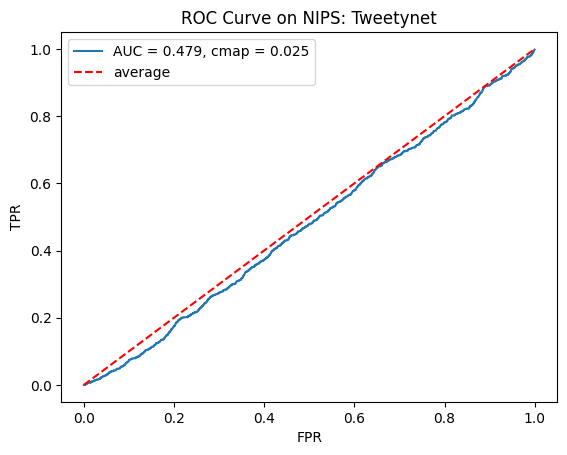
\includegraphics[width=\textwidth]{images/pe_twt_nips_lenient.png}
        \end{column}
        \begin{column}{0.5\textwidth}
            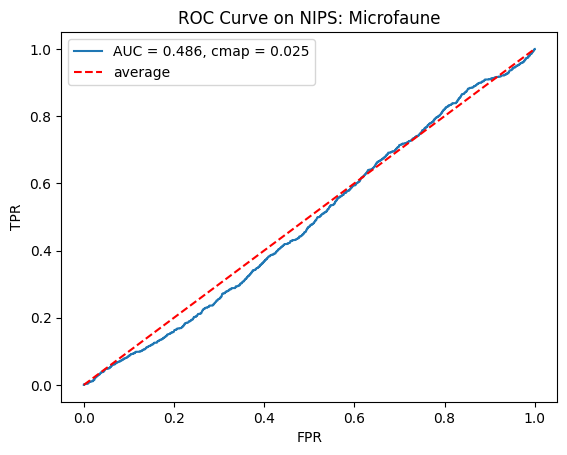
\includegraphics[width=\textwidth]{images/pe_mf_nips_lenient.png}
        \end{column}
    \end{columns}
    Awful performance: Something is wrong with testing!
\end{frame}


\begin{frame}{Sean' updates}
    \begin{enumerate}
        \item Move towards focus primarly on Datasets
        \item Dataset development isn't blocker to model training
        \item Foundational Model Updates delayed
        \item ERSP: Sanity checks complete! Moving onto ML soonish
        \item DSC-MAS: Model development has begun
    \end{enumerate}
\end{frame}
